
\chapter{Introduction to Open Quantum Systems Theory}\label{cap:oqs}

This chapter introduces how quantum systems evolve in time. We begin discussing the unitary evolution of closed quantum systems in Sec. \ref{sec:close}. However, this description cannot be applied to open quantum systems. A solution for this is presented in Sec. \ref{sec:open}, where we present a Markovian master equation and specify its form to describe a thermalisation process. The content of this chapter are based on Refs. \cite{petruccione-book, scully-book, rivas-2010}.



\section{Dynamics of Close Quantum Systems} \label{sec:close}
%Close Quantum Systems Evolution and motivation for OQS
% 1. eq de schrodinger + sistemas fechados ideais
% 2. estados puros vs mistura estatistica = introduzir density matrices
% 3. Liouville-von Neumann
% 4. por que falha para sistemas abertos? perda de unitariedade

Quantum mechanics was initially formulated for isolated systems, whose physical states are represented as a normalised vector $\ket{\psi}$ in the Hilbert space $\mathcal{H}$. This representation contains all the information about the physical state, called a pure state. However, another mathematically equivalent formulation is more convenient for describing quantum systems whose states are not fully known. In these cases, it is only possible to assign a probability $p_i$ of the system existing in the state $\ket{\psi_i}$, which is encapsulated in the density operator,
\begin{equation}
    \hat{\rho} = \sum_i p_i \ket{\psi_i} \bra{\psi_i}.
\end{equation}

\noindent The pure state is a special case in the density operator notation, where it is written as $\hat{\rho} = \ket{\psi}\bra{\psi}$. The density operator (also called density matrix) must satisfy the following conditions: (1) the sum of all $p_i$ is equal to one, which is equivalent to $\text{Tr}[\hat{\rho}] = 1$, and (2) it is positive semi-definite, which means all $\hat{\rho}$ eigenvalues are $\lambda_k \geq 0$.

More than describing physical states, quantum mechanics explains how quantum systems evolve in time. For closed quantum systems, the time evolution is given by the Schrödinger equation,
\begin{equation}
    i \hbar \frac{d}{dt} \ket{\psi (t)} = \hat{H}(t) \ket{\psi (t)},
\end{equation}
\noindent where $\hat{H}(t)$ is the system's Hamiltonian and Planck's constant will be $\hbar = 1$ from now on. This equation can be translated into the density matrices notation as the Liouville-von Neumann equation,
\begin{equation}
    \frac{d}{dt} \hat{\rho}(t) = - i [\hat{H}(t), \hat{\rho} (t)].
\end{equation}

\noindent Its solution describes the unitary evolution of an initial state $\hat{\rho}(0)$ as
\begin{equation}
    \hat{\rho}(t) = U(t) \hat{\rho} (0) U^\dagger (t),
\end{equation}

\noindent where $U(t)$ is a unitary operator with properties $U^{-1} = U^\dagger$ and $U U^\dagger = \mathbb{I}$, in which $\mathbb{I}$ is the identity matrix. Unitary dynamics conserve the total probability, which makes sense as an isolated system cannot lose any information. A consequence of preserving the information is that the dynamics are time-reversible.

Even though all this formalism describes a variety of quantum phenomena, it is an idealisation because every physical system interacts with others. So, let's take a step forward and consider a quantum system ($S$) interacting with another system called the environment ($E$). Together, they form a closed quantum system that evolves in time by the unitary dynamics described before. The total system ($S+E$) is defined by the Hamiltonian
\begin{equation}
    \hat{H}_{SE} = \hat{H}_S \otimes \mathbb{I}_E + \mathbb{I}_S \otimes \hat{H}_E + \hat{H}_I,
\end{equation}

\noindent where $\hat{H}_S$ is the system's Hamiltonian, $\hat{H}_E$ is the environment's Hamiltonian, and $\hat{H}_I$ describes the system-environment interaction. Some characteristics of the environment are that it does not evolve with time and is usually considered to have infinite degrees of freedom, over which we cannot access information or have control. As a result, the system $S$ is the only part we can manipulate, being the focus of our studies. However, because the system $S$ exchanges information with the environment, it does not have a unitary dynamics in general. This is what we call an open quantum system, illustrated in Fig. \ref{fig:oqs-scheme}, whose dynamics will be introduced in the next section.

\begin{figure}[b!]
    \centering
    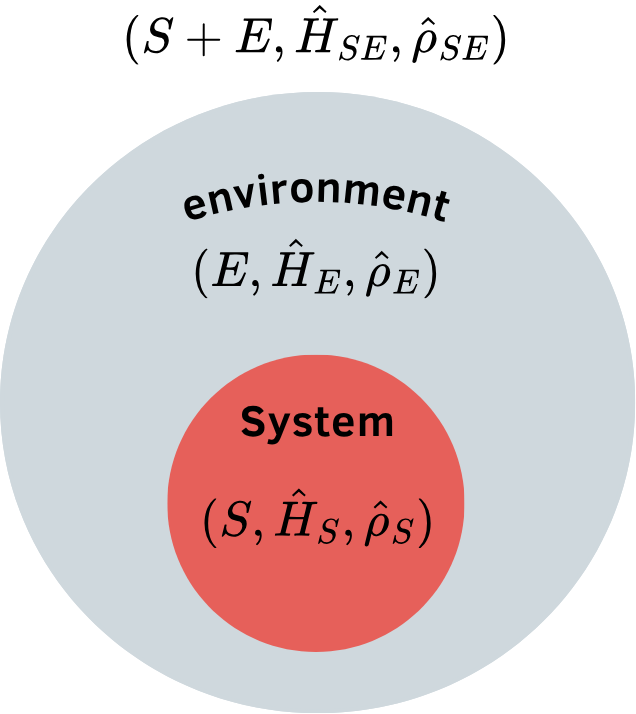
\includegraphics[width=0.35\linewidth]{Images/open-systems-scheme.png}
    \caption{Scheme of an open quantum system.}
    \label{fig:oqs-scheme}
\end{figure}


\section{Dynamics of Open Quantum Systems} \label{sec:open}
%Derivation of Master Equations (Markovian approximation and weak-coupling)
%Davies Map

In this section, we discuss the fundamental steps to obtain the Gorini-Kossakowski-Sudarshan-Lindblad (GKSL) master equation, also called the Lindblad master equation for short. Let's begin with the time evolution of the total system ($S+E$). We know it is unitary, meaning that the Liouville-von Neumann equation can be used. However, we do not have access to all the information in the environment, and including its dynamics in the calculation can be overwhelming. Fortunately, it is possible to make some approximations to describe the system's dynamics, taking into account environmental effects, without needing to deal with the environment's time evolution. These approximations become a bit easier in the interaction picture, where both states and operators change with time. Up to this point, we have used the Schrödinger picture, in which the state evolves with time while the operators remain unchanged. To convert from the Schrödinger picture to the interaction picture, we split the total Hamiltonian as $H_{SE} = H_0 + H_I$ with $H_0 = \hat{H}_S \otimes \mathbb{I}_E + \mathbb{I}_S \otimes \hat{H}_E$, and the time evolution of an operator $\hat{O}$ becomes $\hat{O}(t) = e^{iH_0 t} \hat{O} e^{-iH_0 t}$. As a result, the Liouville-von Neumann equation describing the total system-environment dynamics becomes
\begin{equation}
    \frac{d}{dt} \hat{\rho}_{SE}(t) = -i [\hat{H}_I (t), \hat{\rho}_{SE}(t)].
    \label{eq:neumann-diferencial}
\end{equation}

\noindent We can integrate this equation and substitute into itself, obtaining
\begin{equation}
    \frac{d}{dt}\hat{\rho}_{SE}(t) = -i [\hat{H}_I(t), \hat{\rho}_{SE}(0)] - \int_{0}^{t} ds [\hat{H}_I(t), [\hat{H}_I(s), \hat{\rho}_{SE}(s)]].
\end{equation}

\noindent Because we are only interested in the system's dynamics, we can erase the environment by taking the partial trace. All this algebra still has not solved the problem with environmental dynamics, so our next steps are making approximations. First, we will consider a weak system-environment interaction, allowing us to use the Born approximation, $\hat{\rho}_{SE} (t) \approx \hat{\rho}_S (t) \otimes \hat{\rho}_E$. An interesting consequence of using the weak coupling is that the environment is essentially unaffected by the system $S$, so it can be considered memoryless, allowing us to apply the Markov approximation. In other words, the time the environment takes to erase the system's perturbation is much shorter than the relaxation time, which is equivalent to extending $t \rightarrow \infty$. By using the Markovian approximation, the system's time evolution does not depend on its past states, which means $\rho_S(s) = \rho_S(t)$. After all these approximations, we find the Redfield equation,
\begin{equation}
    \frac{d}{dt} \hat{\rho}_{S}(t) = -i \text{Tr}_E[\hat{H}_I(t), \hat{\rho}_S (0) \otimes \hat{\rho}_E] - \text{Tr}_E\int_{0}^{\infty} ds [\hat{H}_I(t), [\hat{H}_I(s), \hat{\rho}_S (t) \otimes \hat{\rho}_E]].
    \label{eq:redfield}
\end{equation}

\noindent In most cases, the mean of environmental fluctuations is zero, which makes the first term zero. So, we will focus our analysis on the second term.

Although Eq. \eqref{eq:redfield} can describe the relaxation of open quantum systems, it does not guarantee the positivity of probabilities, which can lead to unphysical results. Then, a solution is to use one last approximation: the rotating wave approximation (RWA). In this section, we will use a simpler scenario to make the RWA, but the general case can be found in \cite{petruccione-book}. Let's consider that a perturbation of the bath results in a single effect on the system, that is, no multiple transitions can occur simultaneously in the system. So, the interaction Hamiltonian in the Schrödinger picture can be decomposed into two Hermitian operators as
\begin{equation}
    \hat{H}_I = \hat{A} \otimes \hat{B},
    \label{eq:HI-AkBk}
\end{equation}

\noindent The next step is to write $\hat{A}$ in terms of the eigenstates of the system's Hamiltonian, $\hat{H}_S \ket{n} = \lambda_n \ket{n}$. To make the RWA, we will separate this operator as $\hat{A} = \sum_\omega \hat{A} (\omega)$, where
\begin{equation}
    \hat{A} (\omega) = \sum_{\substack{n,m \\ \omega = \lambda_m - \lambda_n}} \ket{n}\bra{n} \hat{A} \ket{m}\bra{m}
    \label{eq:Ak-w}
\end{equation}

\noindent is summing over all combinations of states that have frequency $\omega$. In the interaction picture, this Hamiltonian becomes
\begin{equation}
    \hat{H}_I (t) = \sum_{\omega} e^{-i\omega t} \hat{A} (\omega) \otimes \hat{B} (t) = \sum_{\omega'} e^{i\omega' t} \hat{A}^\dagger (\omega') \otimes \hat{B}^\dagger (t).
\end{equation}

\noindent The last equality came from using the property $A (\omega) = A^\dagger (-\omega)$ and $\omega' = -\omega$. With this decomposition of the interaction Hamiltonian, we use $s \rightarrow t-s$ and define
\begin{align}
    &\hat{H}_I (t-s) = \sum_{\omega} e^{-i\omega (t-s)} \hat{A} (\omega) \otimes \hat{B} (t-s),\\
    &\hat{H}_I (t) = \sum_{\omega'} e^{i\omega' t} \hat{A}^\dagger (\omega') \otimes \hat{B}^\dagger (t),
\end{align}

\noindent to rewrite Eq. \eqref{eq:redfield} as
\begin{equation}
    \begin{split}
        \frac{d}{dt} \hat{\rho}_{S}(t) &= - \text{Tr}_E\int_{0}^{\infty} ds [\hat{H}_I(t), [\hat{H}_I(t-s), \hat{\rho}_S (t) \otimes \hat{\rho}_E]]\\
        &= \sum_{\omega, \omega'} e^{i (\omega' - \omega)t} \Gamma (\omega) (\hat{A} (\omega) \hat{\rho}_S (t) \hat{A}^\dagger (\omega') - \hat{A}^\dagger (\omega') \hat{A} (\omega) \hat{\rho}_S (t)) + \text{h.c},
    \end{split}
\end{equation}

\noindent where
\begin{equation}
    \Gamma (\omega) = \int_0^{\infty} ds e^{i\omega s} \braket{\hat{B}^\dagger (t) \hat{B} (t-s)}_E,
\end{equation}

\noindent with $\braket{\hat{B}^\dagger (s) \hat{B} (0)}_E = \text{Tr}[\hat{B}^\dagger (s) \hat{B} (0) \hat{\rho}_E]$ being the correlation functions of the bath. The rotating wave approximation imposes that the terms with $\omega \neq \omega'$ oscillate so fast that they do not affect the relaxation process. As a result, only the cases of resonance ($\omega = \omega'$) contribute to the equation. Thus we have
\begin{equation}
    \frac{d}{dt} \hat{\rho}_{S}(t) = \sum_{\omega} \Gamma (\omega) (\hat{A} (\omega) \hat{\rho}_S (t) \hat{A}^\dagger (\omega) - \hat{A}^\dagger (\omega) \hat{A} (\omega) \hat{\rho}_S (t)) + \text{h.c}.
\end{equation}

\noindent One last step to obtain the usual form of the Lindblad master equation is to separate $\Gamma(\omega)$ into its real and imaginary parts as
\begin{equation}
    \Gamma (\omega) = \frac{1}{2} \gamma (\omega) + i S (\omega),
    \label{eq:Gamma-coef}
\end{equation}

\noindent where the transition rate is
\begin{equation}
    \gamma (\omega) = \int_{-\infty}^{\infty} ds e^{i \omega s} \braket{\hat{B}^\dagger (s) \hat{B} (0)}_E,
    \label{eq:gamma-coef}
\end{equation}

\noindent and $S (\omega)$ produce slight changes on the system's energy levels, which are included in the Lamb shift Hamiltonian 
\begin{equation}
    \hat{H}_{LS} = \sum_\omega S (\omega) \hat{A}^\dagger (\omega) \hat{A} (\omega).
    \label{eq:hamiltonian-lamb-shift}
\end{equation}

\noindent As a result, the Lindblad master equation in the interaction picture has the form
\begin{equation}
    \frac{d}{dt} \hat{\rho}_{S}(t) = -i [\hat{H}_{LS}, \hat{\rho}_S (t)] + \mathcal{D}(\hat{\rho}_S(t)),
    \label{eq:lindblad-interaction}
\end{equation}

\noindent with the dissipator being
\begin{equation}
    \mathcal{D}(\hat{\rho}_S) = \sum_\omega \gamma (\omega) \left(\hat{A} (\omega) \hat{\rho}_S \hat{A}^\dagger (\omega) - \frac{1}{2} \{ \hat{A}^\dagger (\omega) \hat{A} (\omega) , \hat{\rho}_S \} \right),
    \label{eq:dissipator}
\end{equation}

\noindent where $\hat{A} (\omega)$ are usually called jump operators. In the Schrödinger picture, the Lindblad master equation becomes
\begin{equation}
    \frac{d}{dt} \hat{\rho}_{S}(t) = -i [\hat{H}_S + \hat{H}_{LS}, \hat{\rho}_S (t)] + \mathcal{D}(\hat{\rho}_S(t)),
    \label{eq:lindblad}
\end{equation}

\noindent where the jump operators remain the same. It is very common to neglect the Lamb shift Hamiltonian, because it only adds a constant to the expression, without changing the physics of the system. That said, from now on, we will use only the $\hat{H}_S$ in our Lindblad master equation.



%%%%%%%%%%%%%%%%%%%%%%%%%%%%%%%%%%%%%%%%%%%%
\subsection{Davies Maps}\label{sec:davies-maps}

An important class of Lindblad master equations is the Davies maps, which generate the thermalisation of a quantum system weakly coupled to a thermal bath at inverse temperature $\beta$ \cite{davies-1979}. This relaxation process always results in thermal states, which means the Davies maps' steady state is always a Gibbs state of the form
\begin{equation}
    \hat{\rho}_{ss} = e^{-\beta \hat{H}_S}/\mathcal{Z}_S,
\end{equation}

\noindent where $\mathcal{Z}_S = \text{Tr}[\exp(-\beta \hat{H}_S)]$ is the partition function. For this to be true, the transition rates $\gamma (\omega)$ must obey the detailed balance condition,
\begin{equation}
    \gamma(-\omega) = \gamma (\omega) e^{-\beta \omega}.
    \label{eq:detailed-balance}
\end{equation}

\noindent Given these conditions, the jump operators of the Davies map have a specific format. Let's rewrite the dissipator (Eq. \eqref{eq:dissipator}) as
\begin{equation}
    \mathcal{D}(\hat{\rho}_S) = \sum_\omega \hat{L}_\omega \hat{\rho}_S \hat{L}_\omega^\dagger - \frac{1}{2} \{ \hat{L}_\omega^\dagger \hat{L}_\omega , \hat{\rho}_S \},
    \label{eq:dissipator-L}
\end{equation}

\noindent defining the jump operators as $\hat{L}_\omega = \sqrt{\gamma (\omega)} \hat{A}(\omega)$. To compute the transition rate ($\gamma (\omega)$), according to Eq. \eqref{eq:gamma-coef}, we need to use that our environment is a thermal bath. The thermal bath can be described by a set of infinite independent harmonic oscillators, $\hat{H}_E = \sum_k \omega_k \hat{b}_k^\dagger \hat{b}_k$, where $\omega_k$ is the frequency of the $k$-mode, and $\hat{b}_k$ and $\hat{b}_k^\dagger$ are the annihilation and creation operators of the $k$-mode. That said, the hermitian operator from Eq. \eqref{eq:HI-AkBk} $\hat{B} = \sum_k (g_k \hat{b}_k^\dagger + g_k^* \hat{b}_k)$ in the interaction picture is
\begin{equation}
    \hat{B} (s) = \sum_k (g_k \hat{b}_k^\dagger e^{i \omega_k s} + g_k^* \hat{b}_k e^{-i \omega_k s}),
\end{equation}

\noindent with $g_k$ being the system-environment coupling parameter. The density matrix of the thermal bath is 
\begin{equation}
    \hat{\rho}_E = \prod_i (1- e^{-\beta \omega_i}) e^{-\beta \omega_i \hat{b}_i^\dagger \hat{b}_i},
\end{equation}

\noindent with which we can compute the correlation functions, obtaining
\begin{equation}
    \braket{\hat{B}^\dagger (s) \hat{B} (0)}_E = \sum_k |g_k|^2 ( e^{-i \omega_k s} (\bar{n}(\omega_k) +1) + e^{i \omega_k s} \bar{n}(\omega_k)),
\end{equation}

\noindent where $\bar{n}(\omega_k) = (e^{\beta \omega_k} -1)^{-1}$ is the Bose-Einstein distribution. Then, we find the transition rates by solving the integral in Eq. \eqref{eq:gamma-coef}, resulting in
\begin{align}
    &\gamma (-\omega) = 2\pi \sum_k |g_k|^2 \bar{n}(\omega_k) \delta(\omega - \omega_k)\\
    &\gamma (+\omega) = 2\pi \sum_k |g_k|^2 (\bar{n}(\omega_k) + 1) \delta(\omega - \omega_k).
\end{align}

\noindent Assuming that the infinite harmonic oscillators of the bath have close frequencies, we can convert from discrete to continuum space by changing the sum to an integral in $\omega$, $g_k$ to a function $g(\omega)$ and including the density function of the bath's states $d(\omega)$. The solution of this new integral gives transition rates that respect the detailed balance (Eq. \eqref{eq:detailed-balance}),
\begin{align}
    &\gamma (-\omega) = \Gamma (\omega) \bar{n}(\omega),\\
    &\gamma (+\omega) = \Gamma (\omega) (\bar{n}(\omega) + 1),
\end{align}

\noindent where $\Gamma (\omega) = 2\pi d(\omega) |g(\omega)|^2$. Considering a homogeneous bath and the same coupling for all $k$-modes, $\Gamma$ becomes a constant. Also, because we have two frequencies, we solve the sum in $\omega$ from the Eq. \eqref{eq:dissipator-L}, obtaining the following Lindblad equation for the Davies maps,
\begin{equation}
    \frac{d}{dt}\hat{\rho}_S (t) = -i [\hat{H}_S, \hat{\rho}_S (t)] + \mathcal{D}^{-} (\hat{\rho}_S) + \mathcal{D}^{+} (\hat{\rho}_S),
    \label{eq:lindblad-davies}
\end{equation}

\noindent where each dissipator's jump operator is
\begin{align}
    &L_\omega^{+} = \sqrt{\Gamma (\bar{n}(\omega)+1)} \hat{A}(\omega),\\
    &L_\omega^{-} = \sqrt{\Gamma \bar{n}(\omega)} \hat{A}(\omega),
\end{align}

After discussing some of the open quantum systems theory, it is always helpful to solve an example. Below, we will solve the thermalisation of a single-mode harmonic oscillator, whose solution will be used later in this work's results.

\subsubsection{Example: single-mode harmonic oscillator coupled to a thermal bath}\label{sec:example}

Consider the system is a single-mode harmonic oscillator $\hat{H}_S = \omega_0 \hat{a}^\dagger \hat{a}$ with $\hat{a}$ and $\hat{a}^\dagger$ being its annihilation and creation operators, respectively. As we discussed before, this system is coupled to a thermal bath of temperature $\beta$, and the relaxation process is described by Eq. \eqref{eq:lindblad-davies}.

Let's find out the jump operators of this case. Usually, the Hermitian operator of the interaction acting on the system subspace is defined as $\hat{A} = \hat{a} + \hat{a}^\dagger$. To decompose $\hat{A}$ into $\hat{A}(\omega)$, we must find out the eigenstates of $\hat{H}_S$ and the frequencies at which this interaction operator makes transitions in our systems. The eigenstates of the harmonic oscillator are Fock states, $\hat{H}_S \ket{n} = \lambda_n \ket{n}$ with $\lambda_n = n \omega_0$. For these states, the creation operator raises one energy level ($\hat{a}^\dagger \ket{n} = \sqrt{n+1} \ket{n+1}$) and the annihilation operator lowers one energy level ($\hat{a} \ket{n} = \sqrt{n} \ket{n-1}$) Using that the energy difference is given by $\lambda_m - \lambda_n = (m - n) \omega_0$, the possible transition frequencies are $+\omega_0$ or $-\omega_0$. Then, the terms of the decomposition of $\hat{A}$ according to Eq. \eqref{eq:Ak-w} becomes
\begin{align}
    &\hat{A}(+\omega_0) = \sum_{m} \ket{m-1}\bra{m-1} \hat{A} \ket{m}\bra{m} = \hat{a},\\
    &\hat{A}(-\omega_0) = \sum_{m} \ket{m+1}\bra{m+1} \hat{A} \ket{m}\bra{m} = \hat{a}^\dagger.
\end{align}

\noindent As a result, the jump operators of this thermal relaxation are
\begin{align}
    &L_\omega^{+} = \sqrt{\Gamma (\bar{n}(\omega)+1)} \hat{a},\\
    &L_\omega^{-} = \sqrt{\Gamma \bar{n}(\omega)} \hat{a}^\dagger.
\end{align}

\noindent This example is fundamentally related to Gaussian states, which will be introduced in Sec. \ref{sec:gaussian}. In Sec. \ref{sec:result-gaussian}, we will analytically solve this master equation.

